\documentclass[12pt, letterpaper]{article}
\usepackage[utf8]{inputenc}
\usepackage{graphicx}
\usepackage{hyperref}
\usepackage{fancyvrb}
\usepackage{array}


\title{Rapport de projet : Bibliothèque génerale au developpement de jeux de Carte}
\author{Vincent AUCONIE \& Chaolei CAI
\\ 
  \multicolumn{1}{
      p{.7\textwidth}}{\centering\emph{Université de Paris \\
  UFR Informatique\\}
  M1 Informatique}
}

\date{\today}

\begin{document}


\begin{titlepage}
    \maketitle
\end{titlepage}

\tableofcontents

\section{Avant propos}
Notre projet est donc de développer un framework général qui permet de géneraliser certaines tâches lors 
du developpement d'un jeu de carte. \\
Un README.ME est inclus dans le fichier, il contient quelques explications quand à l'utilisation et la compilation de la bibliothèque ainsi que les jeux que 
nous avons développés.\\
Il existe un dépôt github si jamais vous avez un souci avec le dossier .zip ou .rar\\
\url{https://github.com/bk211/Projet-POO-M1}

\subsection{Compatibilité et environnement}
La bibliothèque ainsi que les jeux ont été développés en intégralité sous le standard c++11, avec le compilateur g++.
Il est livré sans warning, sans bug(enfin nous l'esperons).\\ 
Niveau compatibilité, cela ne devrait pas poser de problème que vous soyez sous Linux ou windows.\\
Sur la plateforme Windows, l'usage de PowerShell est déconseillé car certaines commandes make ne sont pas exécutable depuis ce shell. 
Utilisez plutôt un shell type git-bash ou cgywin.


\section{Présentation de la bibliothèque}
Le premier point important qui caractérise notre bibliothèque est qu'il est polymorphique dans son intégralité et qu'il est modulable dans une 
très grand partie des cas. \\
Il y a un cadre MVC qui présenté mais vous pouvez tout à fait se contenter d'utiliser seulement les classes containers.\\
Si vous avez besoin d'apporter une spécification à certaines composante, vous êtes libre voir encouragé à le faire ainsi.\\
e.g: vous avez crée une classe UnoCard pour le jeu de uno, vous pouvez tout à fait garder la classe CollectionCarte comme containers de base, 
il sera parfaitement opérationnel. Si vous avez besoin d'un containers plus spécifique à une des besoins, vous pouvez aussi crée votre propre CollectionCarte comme UnoCollectionCarte par exemple.


\subsection{Un ami qui vous veut du bien: Parseur}
D'abord, je m'excuse auprès des plus pointilleux, car le terme Parseur est un peu exagéré en vue de sa fonction.\\
Néanmoins c'est un outil très pratique pour gérer les configurations initiales pour un jeu.\\
Il permet de lire un fichier (.txt) et de convertir son contenu en une matrice de chaînes de charactères.\\
Pour être précis, c'est un vecteur<vecteur<string>>, la séparation des string utilise le symbole de la virgule "," comme délimiteur.
Le désavantage c'est que je n'ai pas fourni de possibilité d'échape à la virgule, donc
la virgule a un usage unique.\\
e.g de démo: \\
considerez le fichier suivant :\\
un,deux,3,quatre,\\
foo,bar,55,zda,\\
lorem,ipsum,42,ws,\\

Le résultat est donc le matrice suivant:\\
\begin{tabular}{l|l|l|l}
  indice[0]  & indice[1] & indice[2] & indice[3]\\
  \hline  
  un & deux & 3 & quatre\\
  \hline
  foo & bar & 55 & zda\\
  \hline
  lorem & ipsum & 42 & ws\\
\end{tabular}
\\
Rien ne vous empêche, au niveau des dimension, de faire des lignes et colonnes irrégulière selon vos désires.\\
Tant que vous savez quoi en faire après.
C'est donc un outil très pratique qui permet d'instancier un deck de jeu selon un fichier de configuration prédefini par exemple.


\subsection{Classe fondamentale: Carte}
La classe Carte est notre structure de donnée qui permet d'en faire une abstraction simpliciste de l'objet Carte.
Elle est apte au polymorphisme. Nous avons enlevé certains getter et setter afin d'être plus lisible. 
A priori, elle couvre déja une très grande partie des besoins pour la plupart des jeux de cartes.\\


\begin{Verbatim}[numbers=left,xleftmargin = 5mm]
class Carte
{
private:
protected:
  std::string name;
  std::vector<std::string> attributs;
  int status;
  int value; 
public:
  virtual ~Carte();
  virtual std::string toString() const;
  friend const std::ostream& operator<<(std::ostream& out, const Carte& mat);
  virtual int operator==(Carte second);
  virtual int operator==(std::string name);
  Carte();
  Carte(std::string name, int status =0, int value = 0);

};
\end{Verbatim}

\subsection{Conteneur de Carte : CollectionCarte }
La classe CollectionCarte est notre classe conteneur de prédilection pour stocker un objet de classe Carte ou sa classe fils.\\
Il permet quelques opérations très pratiques et fréquentes lors d'usage d'un deck de carte comme par exemple mélanger, tirer la première/dernière/au hasard carte
ou encore accèder à une carte d'emplacement précis.

\begin{Verbatim}[numbers=left,xleftmargin = 5mm]
  class CollectionCarte
  {
  protected:
    std::vector<Carte *> data;
  public:
    ...
\end{Verbatim}
 
\subsection{Le joueur}
La classe joueur correspond à notre instance qui permet de représenter un joueur. Il ne possède par défaut qu'une seule main (collection de carte),
mais vous pouvez toujours créer votre propre classe Joueur qui possède plusieurs conteneurs.

\begin{Verbatim}[numbers=left,xleftmargin = 5mm]
class Player{
protected:
    std::string name;
    int status;
    int classId;
    int score;
    CollectionCarte * hand;
    ...
\end{Verbatim} 

\subsection{Conteneur de joueur : PlayerManager}
PlayerManager est notre classe conteneur pour stocker des joueurs, peu importe sa classe.\\
Il permet aussi de gérer certains mécanismes à votre place comme la mémorisation du joueur qui est entrain de jouer 
ou encore de passer au joueur suivant.

\begin{Verbatim}[numbers=left,xleftmargin = 5mm]
class PlayerManager{
protected:
public:
    PlayerManager();
    virtual ~PlayerManager();
    std::vector<Player *> players;
    int currentPlayer;
    int lastPlayer;
    int direction;
    int step;
    ...
    virtual  void swapDirection();
    virtual void setStep(unsigned int s);
    virtual void rotateToNext();
    virtual int nbPlayers();
    ...    
};

\end{Verbatim} 


\subsection{MVC or not MVC? That's The Question}

La bibliothèque propose un cadre MVC presque prêt à l'emploi. A vous de voir si ce cadre vous convient ou non.\\
Les classes Controller et View étant très simple, je ne les détaillerai pas ici.\\
Pour la classe GameModele, il y a une fonction virtuelle pure, il faut donc les implémenter ou juste donner une définition triviale si vous n'en avez pas besoin.\\
Pour cette fonction virtuelle pure pushDataFromStrLine, elle prend en entrée un vecteur de string et ne retourne rien.
Son but est d'instancier les bonnes Cartes nécessaires au jeu selon l'argument donné (Parseur) ? 
C'est ici qu'il donnera petit à petit l'intégralité de son contenu, ligne après ligne.\\

\begin{Verbatim}[numbers=left,xleftmargin = 5mm]
class GameModel{
protected:
    CollectionCarte * data;
    PlayerManager * playerManager;
    GameView * gameView;
    GameController * gameController;
    
public:
    GameModel();
    virtual int initGameData(std::vector<std::vector<std::string>> configData);
    virtual void pushDataFromStrLine(std::vector<std::string> line) = 0;
    virtual void initPlayers();
    virtual void startGame() ;
    ...
};
\end{Verbatim} 



\section{Diagramme UML}
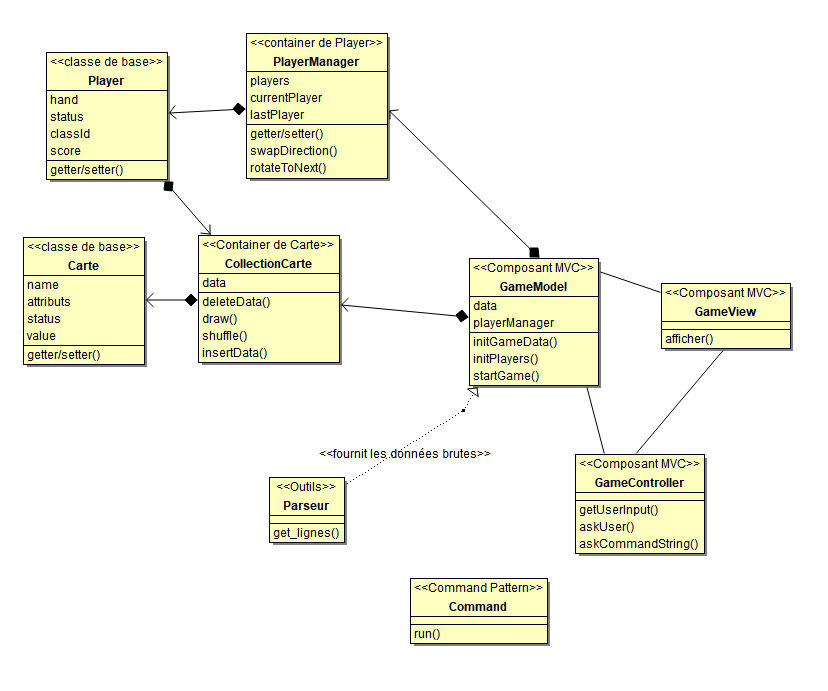
\includegraphics[width=\linewidth]{Diagramme.PNG}

\section{Présentation du jeu Uno realisé grâce à notre bibliothèque}
\subsection{Démarches de developpement}
Pour le jeu Uno nous avons décidé d’utiliser le cadre MVC que proposait notre bibliothèque.
Le début était plutôt simple car pour créer le deck de jeu, nous avions juste à écrire notre définition de pushDataFromStrLine \\

Nous avons aussi créé une classe UnoCard. Ce n’était pas si nécessaire mais cela apportait plus de visibilité à la structure de données,
plutôt que d’utiliser le vecteur de chaînes de charactere fourni par la classe Carte.\\
Une fois l’initiation faite, nous avions plus qu’à écrire la boucle de jeu principale. J’ai du coup employé le Command Pattern dans ce but.\\
Le déroulement est très simple, afficher d’abord les informations utiles (comme la main du joueur qui est en train de jouer).\\
Puis, nous proposons au joueur de choisir une action qu’il souhaite exécuter.\\
Enfin, nous retrouvons la bonne classe Command qui est associée à cette action.\\
Pour le Uno, l’utilisateur pouvait choisir entre "piocher", "jouer une carte" et "crier Uno".\\
Pour chaque action il existe alors une classe Command qui lui était associée.\\
Ainsi nous pouvions nous permettre de nous concentrer sur l’action précise au lieu de tomber dans des boucles logiques de jeu interminable.\\
Cela apporte donc une meilleur visibilité, compréhension du code et une certaine modularité lors du développement.\\

A vrai dire, nous n’avions pas besoin, pour ces jeux, d’une architecture MVC très sophistiquée. Cependant, si on pense les choses un peu plus loin, cela est bénéfique. 
Imaginons qu’on décide un jour d’apporter une interface graphique à notre jeux. Alors, grâce à notre vue, le code du projet se modifiera que très peu. 
Nous aurons juste besoin de changer la méthode d'affichage de notre vue.\\

\subsection{Diagramme de classe de UNO}

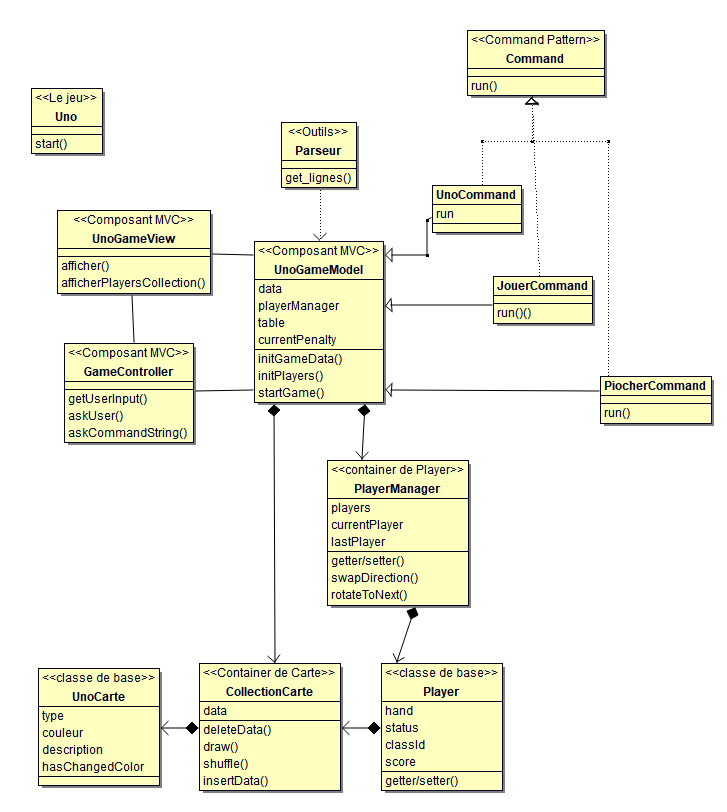
\includegraphics[width=\linewidth]{uno.PNG}
 
\section{Briscola : Cartes différentes mais implémentation identique}
\subsection{Démarches de developpement}
L'implémentation du jeu de la Briscola a révélé quelques différences sur certains points.\\

$\bullet$ Un jeu de cartes différent : Ce changement est en réalité très facile à implémenter grâce à la présence de notre parseur.\\
Il nous a donc suffit de rédiger notre source (.txt) de manière à retrouver les attributs dont nous avions besoin.\\
De plus, la hiérarchie des cartes n'étant pas triviale (le 3 est la deuxième carte la plus forte derrière l'As), nous avons ajouté un attribut de hiérarchie (10 = carte la plus forte, 1 = carte la moins forte) à notre deck.\\
La Briscola nécessitant en plus un comptage des points selon la valeur des cartes, nous avons ajouté un attribut supplémentaire concernant cela.\\

$\bullet$ Le système de manche répétées : Contrairement au Uno, la partie n'est pas continue jusqu'au moment ou un joueur va se débarasser de l'ensemble de ses cartes.\\
En effet, le jeu est séparé en plusieurs manches durant lesquelles chaque joueur va jouer une et une seule fois. Ensuite, l'ordre n'est jamais modifié mais le premier joueur à jouer
est celui ayant gagné la manche précédente. Nous avons alors implémenté une variable permettant de stocker l'information sur le gagnant de la manche pendant son déroulement.\\

$\bullet$ Hormis ces légères différences et d'autres pouvant exister entre les autres jeux, l'implémentation de notre framework nous permet de ne pas avoir à effectuer de trop nombreux changements.

\end{document}
